%% abtex2-modelo-trabalho-academico.tex, v<VERSION> laurocesar
%% Copyright 2012-<COPYRIGHT_YEAR> by abnTeX2 group at http://www.abntex.net.br/ 

\documentclass[
	% -- opções da classe memoir --
	12pt,				% tamanho da fonte
	oneside,			% para impressão mudar para twoside para facilitar impressaõ de frente e verso 
	a4paper,			% tamanho do papel. 
	chapter=TITLE,
	sumario=tradicional,
	% -- opções do pacote babel --
	english,			% idioma adicional para hifenização
	brazil				% o último idioma é o principal do documento
]{abntex2}

% ----------------------------------------------------------
% IMPORTAÇÃO DE PACOTES
% ----------------------------------------------------------
\usepackage{helvet}
\renewcommand{\familydefault}{\sfdefault}			% Usa a fonte Arial			
\usepackage[T1]{fontenc}		% Selecao de codigos de fonte.
\usepackage[utf8]{inputenc}		% Codificacao do documento (conversão automática dos acentos)
\usepackage{indentfirst}		% Indenta o primeiro parágrafo de cada seção.
\usepackage{color}				% Controle das cores
\usepackage{graphicx}			% Inclusão de gráficos
\usepackage{microtype} 			% para melhorias de justificação
\usepackage{hyperref}
\usepackage{times}
\usepackage{siunitx}

\usepackage{amsmath}
\usepackage{amsthm,amsfonts}

\usepackage{lipsum}				% para geração de dummy text
\usepackage{import}
\usepackage{blindtext}
\usepackage{soul}
\usepackage{lscape}

\usepackage{float}


\graphicspath{ {./images/} }

% ---
% Pacotes de citações
% ---
\usepackage[alf]{abntex2cite}	% Citações padrão ABNT

% ----------------------------------------------------------
% CONFIGURAÇÕES DO PDF
% ----------------------------------------------------------

% alterando o aspecto da cor azul
\definecolor{blue}{RGB}{41,5,195}
\definecolor{black}{RGB}{0,0,0}

% informações do PDF
\makeatletter
\hypersetup{
     	%pagebackref=true,
		pdftitle={\@title}, 
		pdfauthor={\@author},
    	pdfsubject={\imprimirpreambulo},
	    pdfcreator={LaTeX with abnTeX2},
		pdfkeywords={abnt}{latex}{abntex}{abntex2}{trabalho acadêmico}, 
		colorlinks=true,       		% false: boxed links; true: colored links
    	linkcolor=black,          	% color of internal links
    	citecolor=black,        		% color of links to bibliography
    	filecolor=black,      		% color of file links
		urlcolor=black,
		bookmarksdepth=4
}
\makeatother

\setlrmarginsandblock{3cm}{2cm}{*}
\setulmarginsandblock{3cm}{2cm}{*}
\checkandfixthelayout

% --- 

% ----------------------------------------------------------
% FIGURAS E TABELAS
% ----------------------------------------------------------

% ---
% Posiciona figuras e tabelas no topo da página quando adicionadas sozinhas
% em um página em branco. Ver https://github.com/abntex/abntex2/issues/170
\makeatletter
\setlength{\@fptop}{5pt} % Set distance from top of page to first float
\makeatother
% ---

% ----------------------------------------------------------
% ESPAÇAMENTOS
% ----------------------------------------------------------

% O tamanho do parágrafo é dado por:
\setlength{\parindent}{1.25cm}

% % Controle do espaçamento entre um parágrafo e outro:
\setlength{\parskip}{0.2cm} 

\setlength{\ABNTEXcitacaorecuo}{4cm}

% Espaçamento entre headers e texto abaixo
\setlength\afterchapskip{0.2cm}
\setlength\aftersecskip{0.2cm} %espaçamento entre seção e texto
\setlength\aftersubsecskip{0.2cm} %espaçamento entre subseção e texto

% ----------------------------------------------------------
% CORREÇÕES DE ESTILO
% ----------------------------------------------------------

% Estilos das legendos
\captionnamefont{\ABNTEXfontereduzida}
\captiontitlefont{\ABNTEXfontereduzida}
\setlength{\belowcaptionskip}{1pt} % espaçamento depois do título das tabelas/figuras
\setlength{\abovecaptionskip}{1pt} % espaçamento antes da legenda de tabelas/figuras

% Estilos dos títulos

\renewcommand{\ABNTEXchapterfontsize}{\bfseries\normalsize}
\renewcommand{\ABNTEXsectionfontsize}{\itshape\normalsize}
\renewcommand{\ABNTEXsubsectionfontsize}{\normalfont\normalsize}
\renewcommand{\ABNTEXsubsubsectionfontsize}{\normalfont\normalsize}

\renewcommand{\chaptitlefont}{\normalfont\bfseries}
\setsecheadstyle{\normalfont\itshape}
\setsubsecheadstyle{\normalfont}
\setsubsubsecheadstyle{\normalfont}

\renewcommand{\ABNTEXchapterfont}{\bfseries}
\renewcommand{\ABNTEXchapterfontsize}{\normalsize}
\setboolean{ABNTEXupperchapter}{true}

% Estilos nos sumários
\renewcommand{\cftchapterfont}{\MakeUppercase}
\setboolean{ABNTEXupperchapter}{true}

\renewcommand{\cftsectionfont}{\normalfont}
\renewcommand{\cftsubsectionfont}{\normalfont}
\renewcommand{\cftsubsubsectionfont}{\normalfont}

% ----------------------------------------------------------
% COMPILA O ÍNDICE
% ----------------------------------------------------------
\makeindex

% ----------------------------------------------------------
% COMANDOS CUSTOMIZADOS
% ----------------------------------------------------------
\newcommand{\un}[1]{\;\text{#1}}
\newcommand{\logo}{\quad \Rightarrow \quad}
\newcommand{\codeword}[1]{\texttt{\textcolor{black}{#1}}}
\newcommand{\specialcell}[2][c]{%
  \begin{tabular}[#1]{@{}c@{}}#2\end{tabular}}

% ----------------------------------------------------------
% INÍCIO DO DOCUMENTO
% ----------------------------------------------------------
\begin{document}

%\selectlanguage{english}
\selectlanguage{brazil}

% Retira espaço extra obsoleto entre as frases.
\frenchspacing 

% ----------------------------------------------------------
% ELEMENTOS PRÉ-TEXTUAIS
% ----------------------------------------------------------
\begin{center}
\textbf{UNIVERSIDADE FEDERAL DE MINAS GERAIS\\
Escola de Engenharia \\
Curso de Bacharelado em Engenharia de Sistemas}

\vspace{4cm}

%\hspace{0.3\textwidth} \parbox{0.65\textwidth}
Cleyton Luan Nobre Assis 2021019815 \\
Maria Clara Oliveira Domingos Ruas 2021019572 \\
Raphael Henrique Braga Leivas 2020028101

\vspace{4cm}  

{ \textbf{Laboratório de Circuitos Eletrônicos e Projetos - Prática 4} }

\vfill
%\hspace{0.3\textwidth} 
{Belo Horizonte \\
2025 }
\end{center}

\newpage

% ---
% inserir o sumario
% ---
\pdfbookmark[0]{\contentsname}{toc}
\tableofcontents*
\cleardoublepage
% ---

% % ----------------------------------------------------------
% % ELEMENTOS TEXTUAIS
% % ----------------------------------------------------------
\textual

\pagestyle{simple}
	
\chapter{Objetivos}\label{cap:objetivos} 

Este relatório é referente à prática 4 da disciplina de Laboratório de Circuitos Eletrônicos I, `` ghihi''.  Como objetivos principais, temos:

\begin{itemize}
    \item Compreender o princípio da proteção grampeada para fontes transistorizadas;
    \item Entender como utilizar o circuito análogo térmico para estimar as temperaturas no transistor e dissipador;
    \item Aplicar amplificadores operacionais como condicionamento de sinais e comparador para detecção de corrente.
    
\end{itemize}


\chapter{Introdução}\label{cap:introdução} 




Durante a prática, ambos os circuitos — proteção grampeada e medição e detecção de corrente — foram montados, testados e simulados no software LTSpice.

\chapter{Desenvolvimento}

O desenvolvimento das atividades da prática foram divididos entre 2 experimentos:
\begin{itemize}
    \item Proteção grampeada
    \item Medição e detecção de corrente

\end{itemize}
Dentro de cada experimento, existe uma explicação breve sobre o procedimento, os resultados obtidos junto com as simulações e cálculos necessários, e por fim uma discussão sobre os resultados obtidos.

\section{Experimento 1}

No experimento 1, vamos verificar como a tensão de Offset é presente na saída do AmpOp mesmo que a tensão de entrada seja zero. O circuito a ser montado 
está exibido na \autoref{fig:exp1_circ}. A montagem em protoboard está exibida na \autoref{fig:exp1_circ_pb}.

\begin{figure}[h!]
	\caption{\label{fig:exp1_circ} Circuito do experimento 1.}
	\begin{center}
    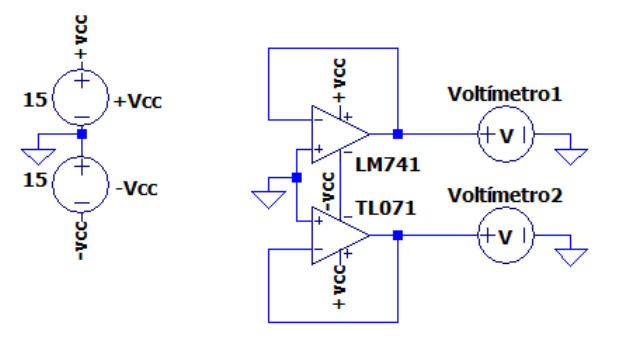
\includegraphics[width=0.5\textwidth,trim=1 1 1 1,clip]{images/Pratica4/exp1_circ.png}
	\end{center}
\end{figure}

\begin{figure}[h!]
	\caption{\label{fig:exp1_circ_pb} Circuito do experimento 1 montado em protoboard.}
	\begin{center}
    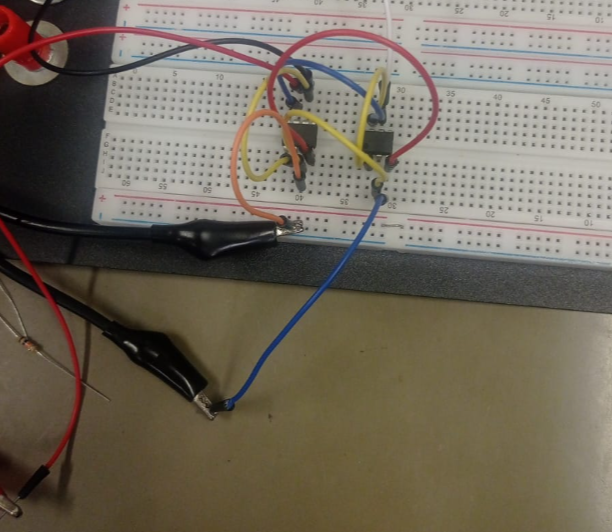
\includegraphics[width=0.6\textwidth,trim=1 1 1 1,clip]{images/Pratica4/exp1_circ_pb.png}
	\end{center}
\end{figure}



\subsection{Resultados Obtidos}

A tensão medida nas saídas dos AmpOps está exibida na \autoref{tab:exp1_res}.

\begin{table}[htb]
	\caption{Valores medidos e esperados (datasheet) da tensão de offset dos AmpOps.}
	\centering
	\begin{tabular}{c|c|c}
		\hline
    		\textbf{AmpOp}  & \textbf{Offset Datasheet (mV)} & \textbf{Offset Medido (mV)} \\
            \hline
    		TL071 & 1 (typ) , 5 (max) & -2.6 \\
            \hline
            LM741 & 3 (typ) , 10 (max) & 2.9 \\
            \hline
	\end{tabular}
	\label{tab:exp1_res}
\end{table}

\subsection{Discussão}

Tendo em vista que a tensão de offset é amplificada junto com o sinal de entrada, para ganhos elevados o 
LM741 apresenta maior necessidade de ajuste do offset, uma vez que ele apresenta uma tensão de offset maior 
em módulo. De fato, se o ganho do circuito for $G = 100$, a tensão de offset na saída já seria 
de 

\[ V_o = 2.9 \un{mV} \cdot 100 = 0.3 \un{V} \]

\noindent um valor que pode ser significativo para certas aplicações.

\section{Experimento 2}


\subsection{Resultados Obtidos}


\subsection{Discussão}

\section{Experimento 3}


\subsection{Resultados Obtidos}


\subsection{Discussão}

\section{Experimento 4}

Usando o mesmo circuito dos experimentos 2 e 3, vamos identificar qual a banda passante 
de cada AmpOp através da forma de onda. Para isso, coloca-se um sinal de entrada com 
frequência de $f = 1 \un{kHz}$ e verificar a tensão de pico a pico. Depois, aumenta-se a 
frequência de entrada até que a tensão pico a pico medida caia em 30\%, representando 
uma queda de -3 dB.


\subsection{Resultados Obtidos}

A \autoref{fig:exp4_1khz} mostra as formas de onda para o LM741 (amarelo) e TL071 (azul)
com o sinal de entrada de $f = 1 \un{kHz}$. Ambos possuem $V_{pp} = 1.88 \un{V}$.

\begin{figure}[h!]
	\caption{\label{fig:exp4_1khz} Saídas do TL071 (azul) e LM741 (amarelo) para um sinal de entrada 
    com $f = 1 \un{kHz}$.}
	\begin{center}
    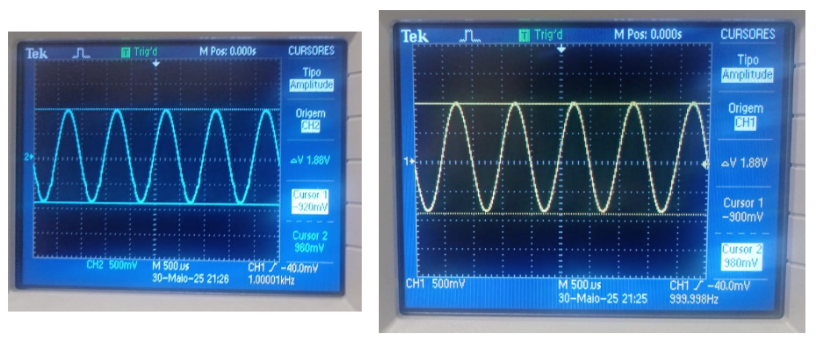
\includegraphics[width=\textwidth,trim=1 1 1 1,clip]{images/Pratica4/exp4_1khz.png}
	\end{center}
\end{figure}

Variando-se a frequência, precisamos obter um sinal com $V_{pp} = 1.88 \cdot 0.7 = 1.3 \un{V}$ 
para identificar a frequência de corte da banda passante de cada AmpOp. As formas de onda da 
\autoref{fig:exp4_corte} foram obtidas respectivamente em $f = 86 \un{kHz}$ (azul, TL071) e 
$f = 83 \un{kHz}$ (amarelo, LM741), indicando que essas são as bandas passantes respectivamente do TL071 a LM741.

\begin{figure}[h!]
	\caption{\label{fig:exp4_corte} Saídas do TL071 (azul) e LM741 (amarelo) para um sinal de entrada 
    com $f = 86 \un{kHz}$ e $f = 83 \un{kHz}$, respectivamente.}
	\begin{center}
    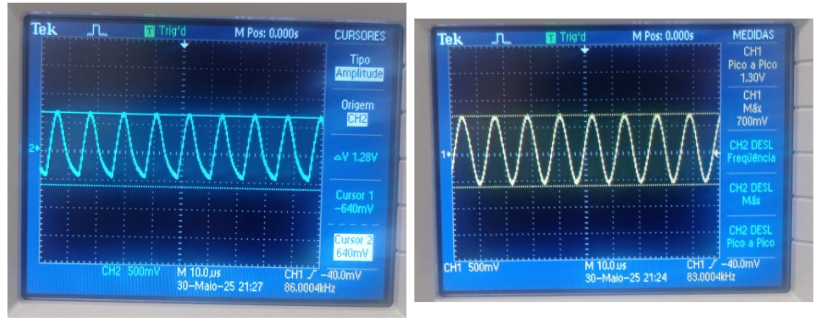
\includegraphics[width=\textwidth,trim=1 1 1 1,clip]{images/Pratica4/exp4_corte.png}
	\end{center}
\end{figure}

\subsection{Discussão}

Os datasheets indicam que as bandas passantes do TL071 e LM741 são na ordem de MHz, 
significativamente maiores que os valores experimentais obtidos na \autoref{fig:exp4_corte}.
Contudo, isso pode ser explicado pelo fato de o teste ter sido realizado em protoboard, 
que possui capacitâncias que atenuam componentes de alta frequência, reduzindo a 
banda passante do circuito.

\chapter{Conclusão}\label{cap:conclusao} 

Tendo em vista os objetivos da Seção \ref{cap:objetivos}, foi possível 

\end{document}
